\documentclass[a4paper,12pt]{book}
\usepackage[margin=2cm]{geometry}		
\usepackage{uglix}
\usepackage{array,numprint}
\usepackage{systeme}
\usepackage{multirow}
\progfonts{0.85}
\setcounter{chapter}{9}
\nouveaustyle
\begin{document}
\titre{Devoir Maison}{SIO2}{04/2020}

\subsection*{Consignes}

Rendre le devoir sur l'espace de restitution de \textsc{Pronote} \textbf{avant le mardi de la rentrée}.\\
Le devoir doit être un document PDF (pas de .doc, .docx, .odt).\\
Pour dessiner des graphes, utiliser yEd, téléchargeable ici :\\ \url{https://www.yworks.com/products/yed#}

\subsection*{\'Enoncé}


\begin{exercice}[ (6 du cours)]
Trouve un chemin hamiltonien, un circuit de longueur 3 et un autre de longueur 4.
\begin{center}
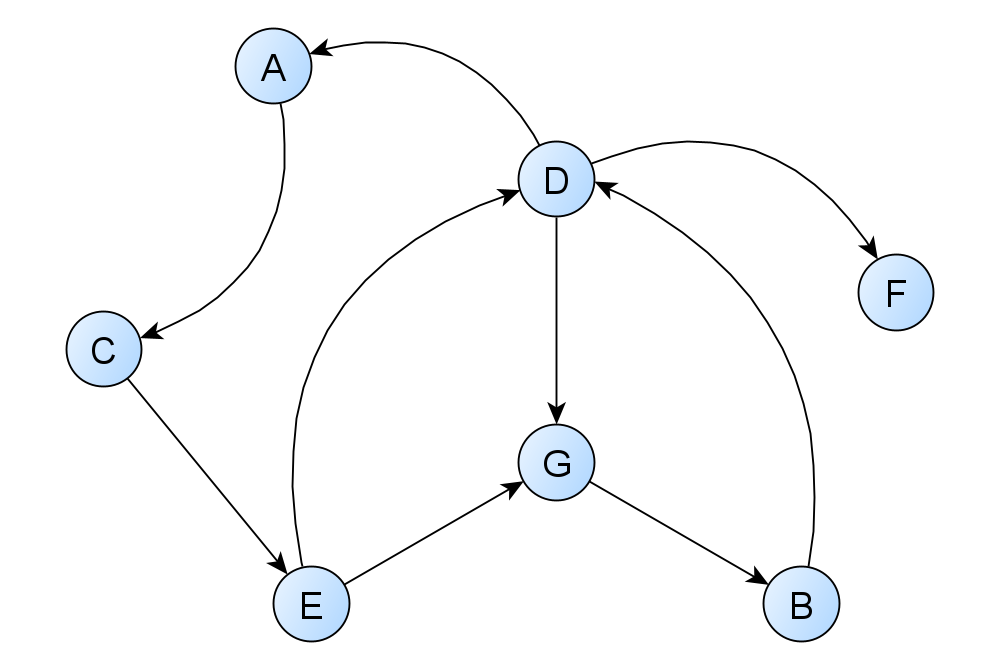
\includegraphics[width=7cm]{img/ex_circuit_ch.png}
\end{center}
\end{exercice}



\begin{exercice}[ (7 du cours)]
On donne le tableau de prédécesseurs suivants :
\begin{center}
\begin{tabular}{|l|>{\centering\arraybackslash}p{1cm}|>{\centering\arraybackslash}p{1cm}|>{\centering\arraybackslash}p{1cm}|>{\centering\arraybackslash}p{1cm}|>{\centering\arraybackslash}p{1cm}|>{\centering\arraybackslash}p{1cm}|}
\hline
sommet		 	& A 	& B 	& C 	& D 	& E 	& F\\
\hline
prédécesseurs 	& --- 	& --- 	& A,B,E & F 	& B,D   & A,B\\
\hline
\end{tabular}
\end{center}
En utilisant les puissances de la matrice d'adjacence :
\begin{enumerate}[--]
	\item 	Donner tous les chemins de longueur 3.
	\item 	Montrer qu'il n'existe pas de chemin de longueur 5.
	\item 	Montrer que ce graphe ne possède pas de circuit.
\end{enumerate}
\end{exercice}

\begin{exercice}[]
Voici un graphe.
\begin{center}
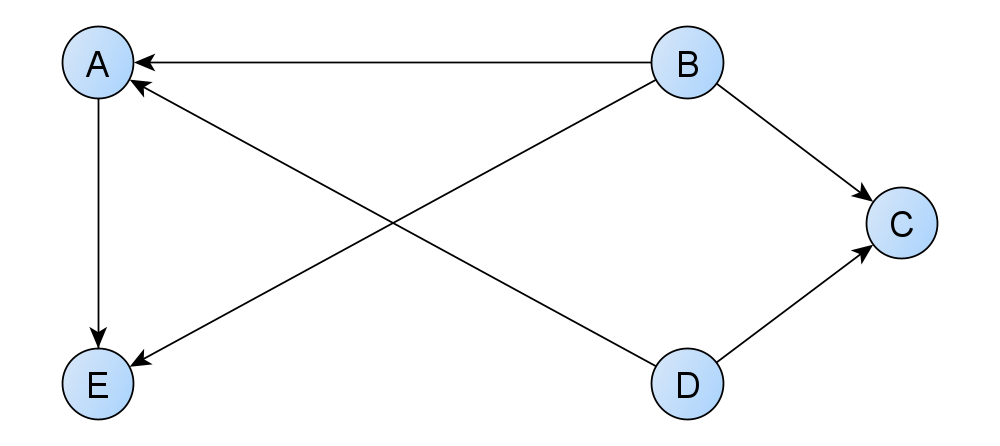
\includegraphics[width=7cm]{img/exo_dm.png}
\end{center}
\begin{enumerate}[\bfseries 1.]
	\item 	Donner M, matrice d'adjacence du graphe.
	\item 	Calculer $\widehat{M}$, matrice de la fermeture transitive de ce graphe.\\
	\item 	Quels arcs doit-on ajouter au graphe ci-dessus pour réaliser sa fermeture transitive ?
\end{enumerate}
\end{exercice}
\end{document}
